%	현대물리실험 보고서
%	실험4
%	202100973 이승엽

%----------------------------------------------------------------------------------------
%	PACKAGES AND DOCUMENT CONFIGURATIONS
%----------------------------------------------------------------------------------------

\documentclass[a4paper, 10pt, nanum]{CSUniSchoolLabReport}
% use UTF8 encoding
\usepackage[utf8]{inputenc}
% use KoTeX package for Korean
\usepackage{kotex}
% use ams' math font
\usepackage{amsmath}
\usepackage{hyperref}
% use table
\usepackage{graphicx}
\usepackage{multirow}
\usepackage{indentfirst}
\usepackage{setspace}
\usepackage{enumitem}
\usepackage{wrapfig}
\usepackage{epstopdf}
% use captions
\usepackage{caption}
\usepackage{subcaption}
\usepackage{blindtext}
% use layout frame
\usepackage{showframe}

% Setting the graphics path
\graphicspath{{Figures/}}

% only for show page layout
\renewcommand\ShowFrameLinethickness{0.25pt}
\renewcommand*\ShowFrameColor{\color{red}}

\setlength{\parindent}{0.2in} % 들여쓰기 길이 설정
\setlength{\parskip}{3mm} % 문단 간의 간격 조절
\setstretch{1.5} % 줄간격
% \graphicpath{{Figures/}} % fig 경로 설정

\addbibresource{reference.bib} % Bibliography file (located in the same folder as the template)

%----------------------------------------------------------------------------------------
%	REPORT INFORMATION
%----------------------------------------------------------------------------------------

\title{현대물리실험 실험4 보고서 \\ Scanning Tunneling Microscope} % Report title

\author{\textsc{Department of Physics} 202100973 이승엽}

\date{\today}

%----------------------------------------------------------------------------------------

\begin{document}

\maketitle % Insert the title, author and date using the information specified above

\begin{center}
	\begin{tabular}{l r}
		Date Performed: & May 16, 2023 \\ % Date the experiment was performed
		& May 23, 2023 \\
		Partners: & 202100969 이규리 \\ % Partner names
		& 202100989 한누리 \\
		Instructor: & Professor 이기주 \\ % Instructor/supervisor
		Typesetting: & LaTeX \\
		Datafitting: & Python \\
	\end{tabular}
\end{center}

%----------------------------------------------------------------------------------------
%	ABSTRACT
%----------------------------------------------------------------------------------------

\maketitle
% \begin{abstract}
% 	This report ...
% \end{abstract}

%----------------------------------------------------------------------------------------
%	INTRODUCTION
%----------------------------------------------------------------------------------------

\section{Introduction}

	Microscopy is one of the most exciting scientific techniques. The insight into small dimensions has led to a new understanding of the structure of materials and forms of life.

	With the help of the scanning tunneling microscope (STM) it is possible to look into the fascinating world of the atoms. This completely new microscopy technique works without focusing elements and features atomic resolution (laterally and vertically).

	The Scanning Tunneling Microscope was developed by Gerd Binnig and Heinrich Rohrer in the early 80’s at the IBM research laboratory in Ruschlikon, Switzerland. For this revolutionary innovation Binnig and Rohrer were awarded the Nobel prize in Physics in 1986.

	In the STM, a small sharp conducting tip is scanned across the sample’s surface, so close that the so-called ”tunneling current”can flow. With the help of that current the tip-sample distance can be controlled very precisely. Therefore an enormous resolution is achieved so that the atomic arrangement of metallic surfaces can be “probed”

	To be able to get such excellent pictures of atomic resolution is almost incredible, considering that the size of the atom in relation to the tip is that of a golf ball to a mountain.
	
	In the NaioSTM, a platinum-iridium tip is moved in three dimensions using piezo crystal translators that are driven with sub-nanometer precision.

	The sample to be examined approaches the tip within a distance of 1 nanometer (1 nm= 1I 1,000,000,000 m). Classical physics would prohibit the appearance of electrons in the small gap between a tip and a sample, but if a sharp tip and a conducting surface are put under a low voltage (U ∼0.1 V), a very small tunneling current (I∼ 1 nA) may nevertheless flow between tip and sample. This tunneling current is due to a quantum physics effect.

	The strength of the tunneling current depends exponentially on the distance between the tip and the sample (usually referred to as Z-Distance). This extreme dependence on the Z-Distance makes it possible to measure the tip-sample movement very precisely. One of the three piezo crystals, the Z-piezo, can now be used in a feedback loop that keeps the tunneling current constant by appropriately changing the Z-Distance.

	To obtain an image of the sample, the tip is scanned using the X- and Y-piezo crystals. The feedback loop will now let the tip follow the structure of the sample's surface. A height image can now be made by recording the position of the Z-feedback loop as a function of the XY-piezo position. This ”landscape” (or topography) of the atomic surface is then drawn line by line on the computer screen.

	The sample can also be scanned in a second mode: When the feedback loop is slowed down very much, the tip scans at a fixed distance from the sample (constant height mode). This time the variations in the tunneling current are measured and drawn line by line on the computer screen. However, this mode only works when the sample is atomically flat, because the tip would otherwise ”crash” into the sample. 


%----------------------------------------------------------------------------------------
%	THEORY
%----------------------------------------------------------------------------------------

\section{Theory}

	STM은 양자 터널 효과(quantum tunneling)의 개념을 기반으로 작동한다. 전도 팁이 측정 대상 표면에 접근할 때, 둘 사이에 가해지는 바이어스(전압 차이)는 전자가 전도팁과 측정대상 표면 사이의 진공 속을 통과하도록 한다. 이 때 발생하는 터널링 전류(전도팁과 표면의 전류)는 팁 위치, 인가 전압 및 샘플 상태(LDOS)에 따라 변화하기 때문에 이를 이용하여 표면의 상태를 영상정보로 변환한다. STM 측정은 표면상태, 팁, 진동제어, 전자장치에 따라 민감한 특성을 보이는 매우 정교한 기술이다.

	\begin{figure}[htb!]
		\centering
		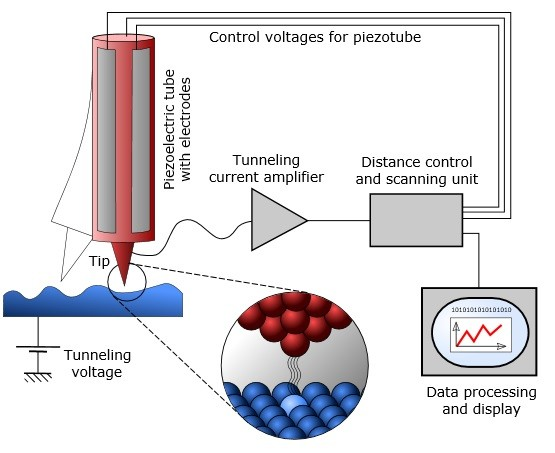
\includegraphics[width=5cm]{Figures/STM1.jpg}
		\caption{Schematic view of an STM.}
		\label{fig:STM}
	\end{figure}

  전압 바이어스를 팁과 샘플 표면에 적용하고 팁을 샘플 표면에 매우 가깝게 접근시킨다. 근거리에서, 표본 가까이에 있는 경우, 일반적으로 팁은 샘플 표면에 인력과 척력이 평형을 이루는 위치(보통 4-7 Å(0.4-0.7 nm))에 놓이게 되고 팁의 위치는 압전(piezoelectric)소재로 구성된 팁의 본체를 통해 전기 신호로 외부 데이터 수집장치 등에 수신하거나, 외부에서 조절될 수 있다. 이것을 증폭기(amplifier)를 통해 조작자가 인식할 수 있도록 한다. 또한 샘플과 팁사이에 흐르는 전류를 이용하여 셈플 표면상태 등을 인식할 수 있다.

	샘플의 표면에서 x-y 평면 방향으로 팁을 이동시키면 표면 높이와 상태 밀도의 변화가 전류 변화가 일어나며 이미지로 매핑하게 된다. 위치에 대한 이러한 전류 변화는 자체적으로 측정가능하며, 일정한 전류에 해당하는 팁의 높이 z또한 측정가능하다. 

	표면을 측정하는 방식은 팁의 높이를 일정하게 유지한 상태에서 전류변화를 감지하는 방법, 표면과 팁의 전류를 일정하게 유지하는 상태에서 팁의 높이를 측정하는 방법이 있다. 일반적으로 높이를 일정하게 유지하는 것이 전류를 일정하게 유지하는 것보다 측정 속력이 빠른 것으로 알려져 있다.

%----------------------------------------------------------------------------------------
%	EXPERIMENTAL METHOD
%----------------------------------------------------------------------------------------

\section{Experimental Method}

\subsection{STM 측정용 팁 만들기}
	\begin{enumerate}[label=\arabic*.]
		\item Pt/Ir wire의 일부를 잘라 사용한다. 가장 어려운 부분이므로 신중하게 한다.
		Magnifying cover를 The NaioSTM system에서 분리한 NaioSTM tool set에서 the wire cutters, the Flat nose pliers 그리고 the pointed tweezers를 에탄올로 닦는다.		
		\item the pointed tweezers를 사용해 '오래된 tip'을 제거한다. 만약, '오래된 tip'이 충분히 길다면 그 '오래된 tip'을 잘라 쓸 수도 있다
		\item tip으로 쓰게 될 와이어를 꺼낸다.
		\item pliers를 왼손에 쥐고 꽉 잡아 흔들리지 않도록 한다.
		\item 그 상태에서 cutters로 약 4 mm정도의 길이로 비스듬히 자른다. 주의할 점은 wire를 싹뚝 잘라내는 것이 아니라 깍아 내듯이 잘라야 한다. tip의 끝이 굉장히 날카로워야 하기 때문에 자르는 것이 아니라 찢어내듯이 잘라야 한다. 그렇지 않으면 선명한 신호를 얻어내지 못한다.
		\item the pointed tweezers를 이용해 The NaioSTM system 본체 안쪽에 고정시킨다. 팁이 0.2~0.3 cm정도 튀어나오도록 장착한다.
		\item Magnifying cover로 닫고 확대경으로 다음과 같이 장착되었는지 팁 끝부분을 확인한다.
		\item 측정샘플을 홀더에 고정하기 위해 NaioSTM tool set에서 홀더를 꺼낸다.
		\item 손에 라텍스 장갑을 써서 샘플이 오염되지 않도록 한다.
		\item NaioSTM tool set에서 트위져와 측정샘플을 꺼내어 홀더에 장착한다. (홀더에 자성으로 고정이 되므로 끝 부분을 잡고 살짝 놓는다.  장갑을 껴도, 샘플 holder의 금속 부분은 만지지 않도록 해야 합니다.)
		\item 측정샘플을 장착한 홀더를 The NaioSTM system헤드에 끼운다.
		\begin{figure}[htb!]
			\centering
			\begin{minipage}{.5\textwidth}
				\centering
				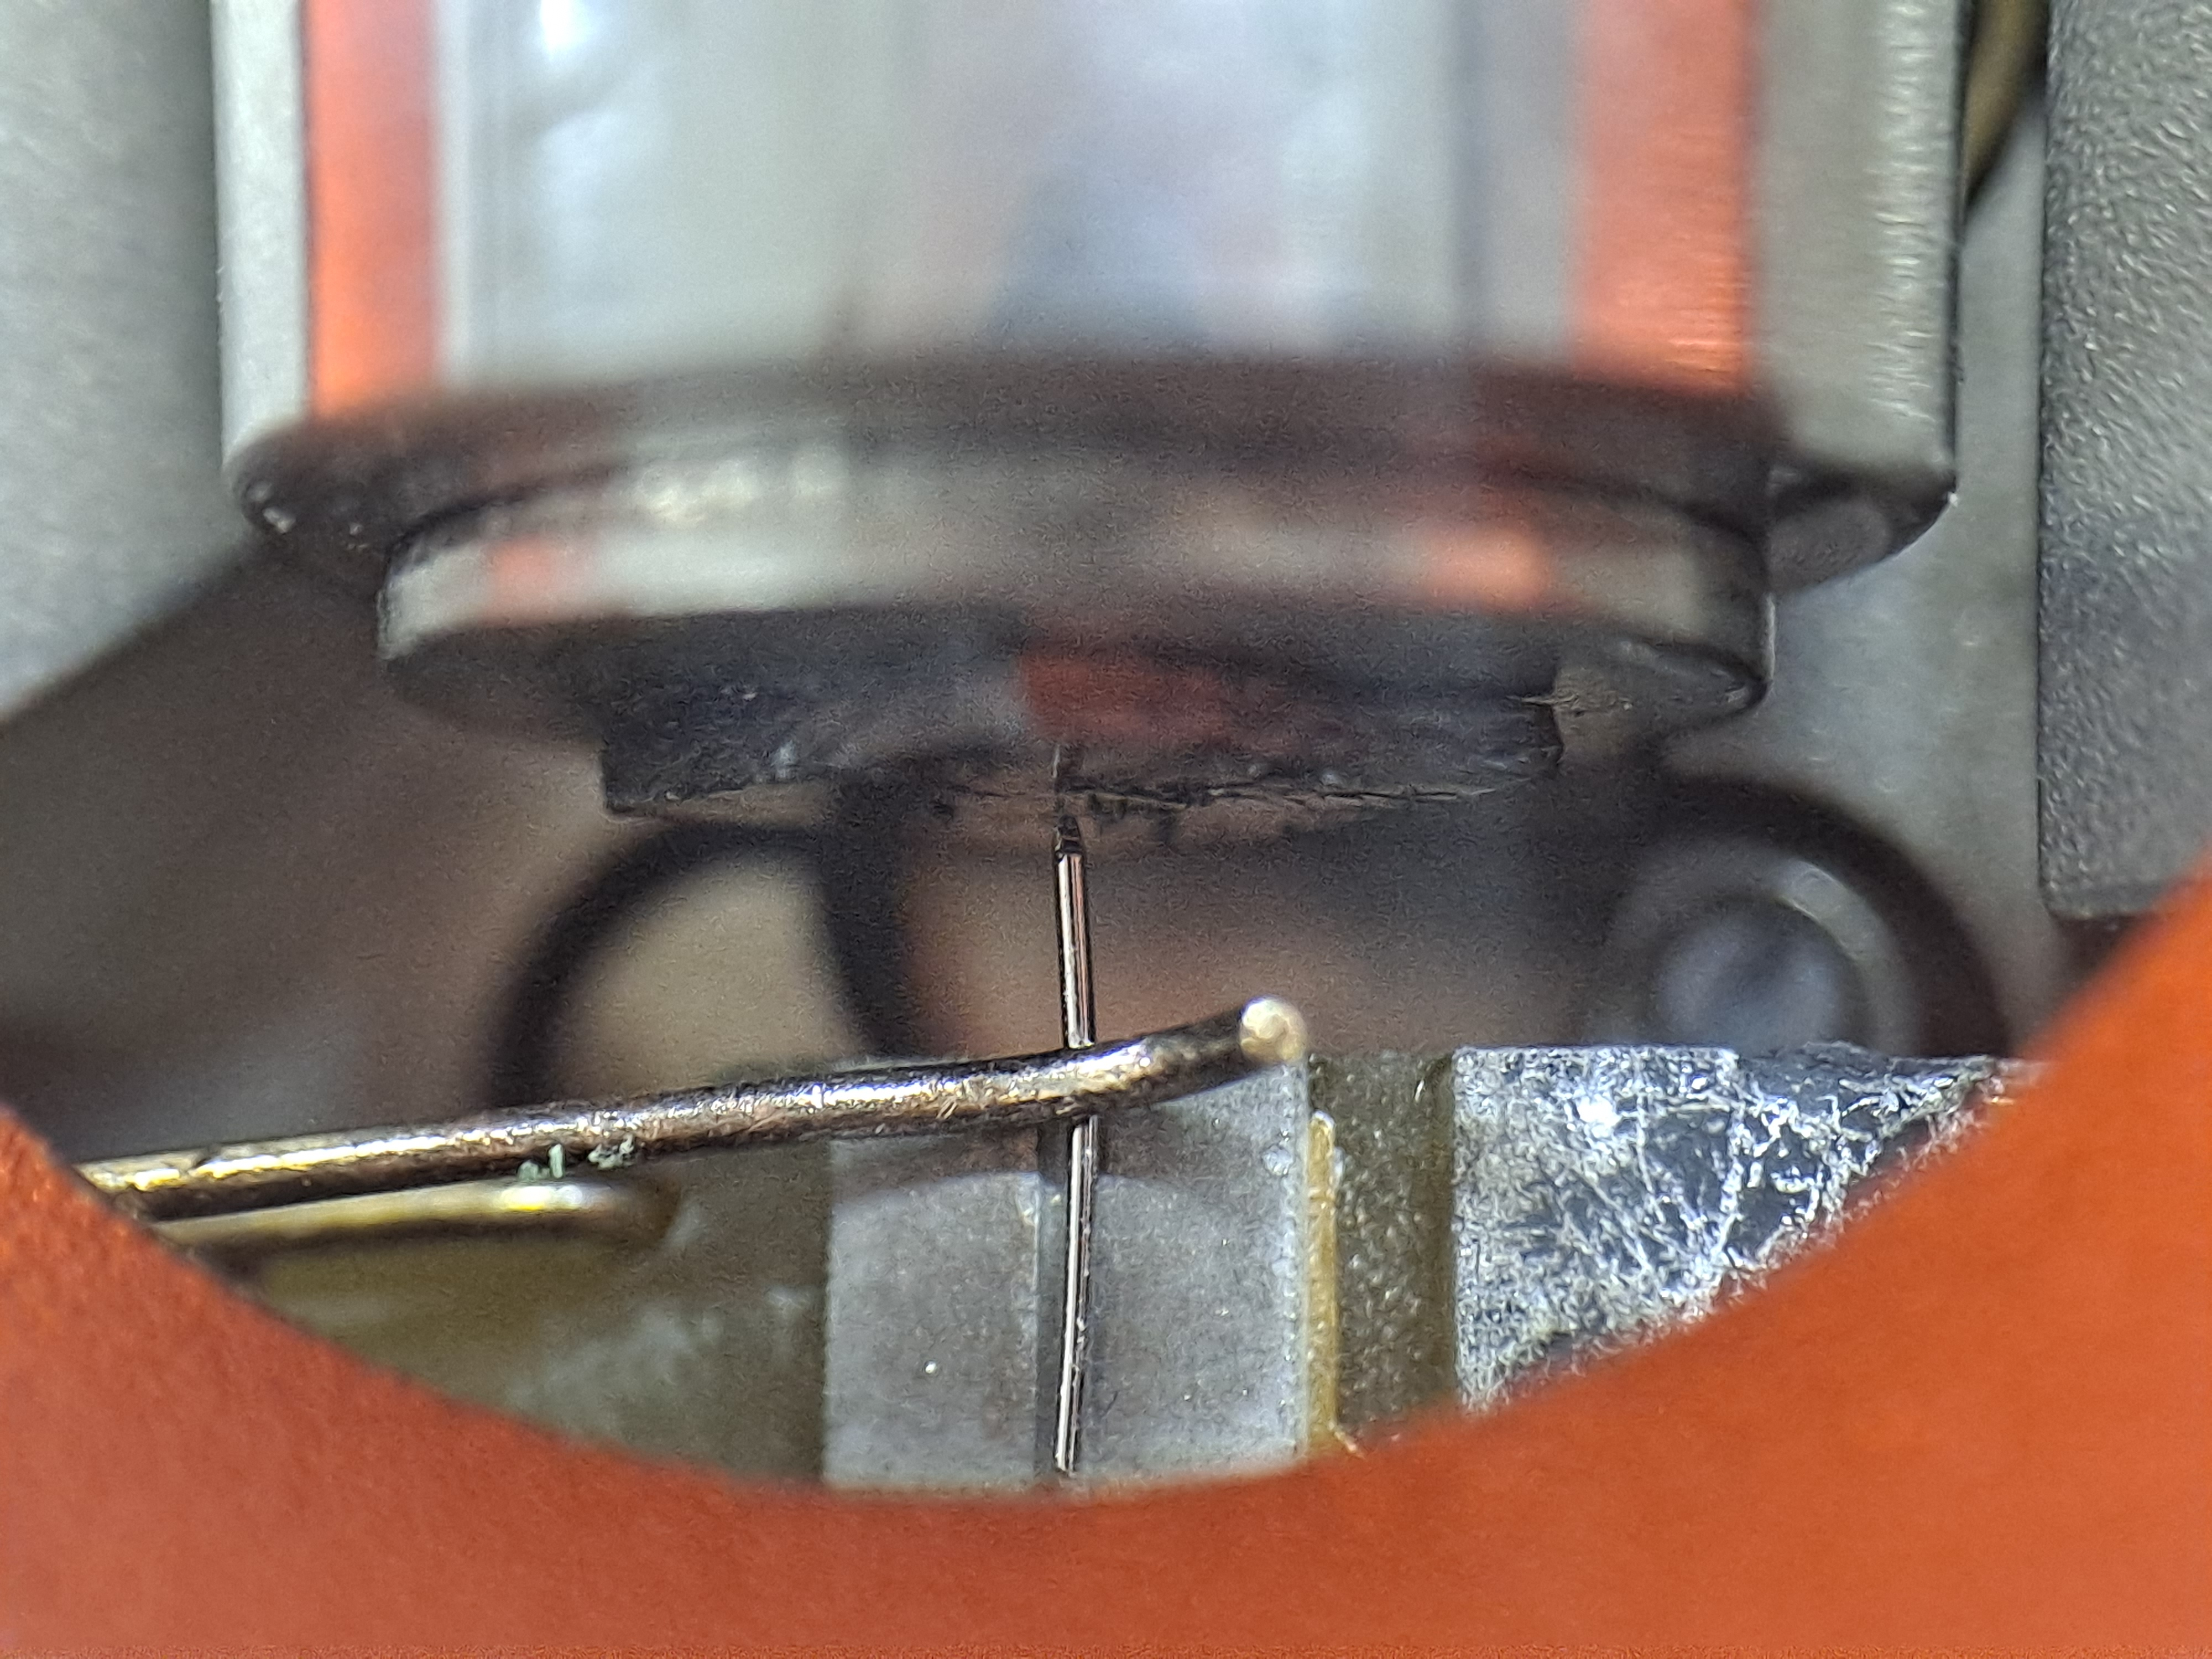
\includegraphics[width=5cm]{Figures/STM_TIP1.jpg}
				\captionof{figure}{Tip mounted on the STM.}
				\label{fig:STM_TIP1}
			\end{minipage}%
			\begin{minipage}{.5\textwidth}
				\centering
				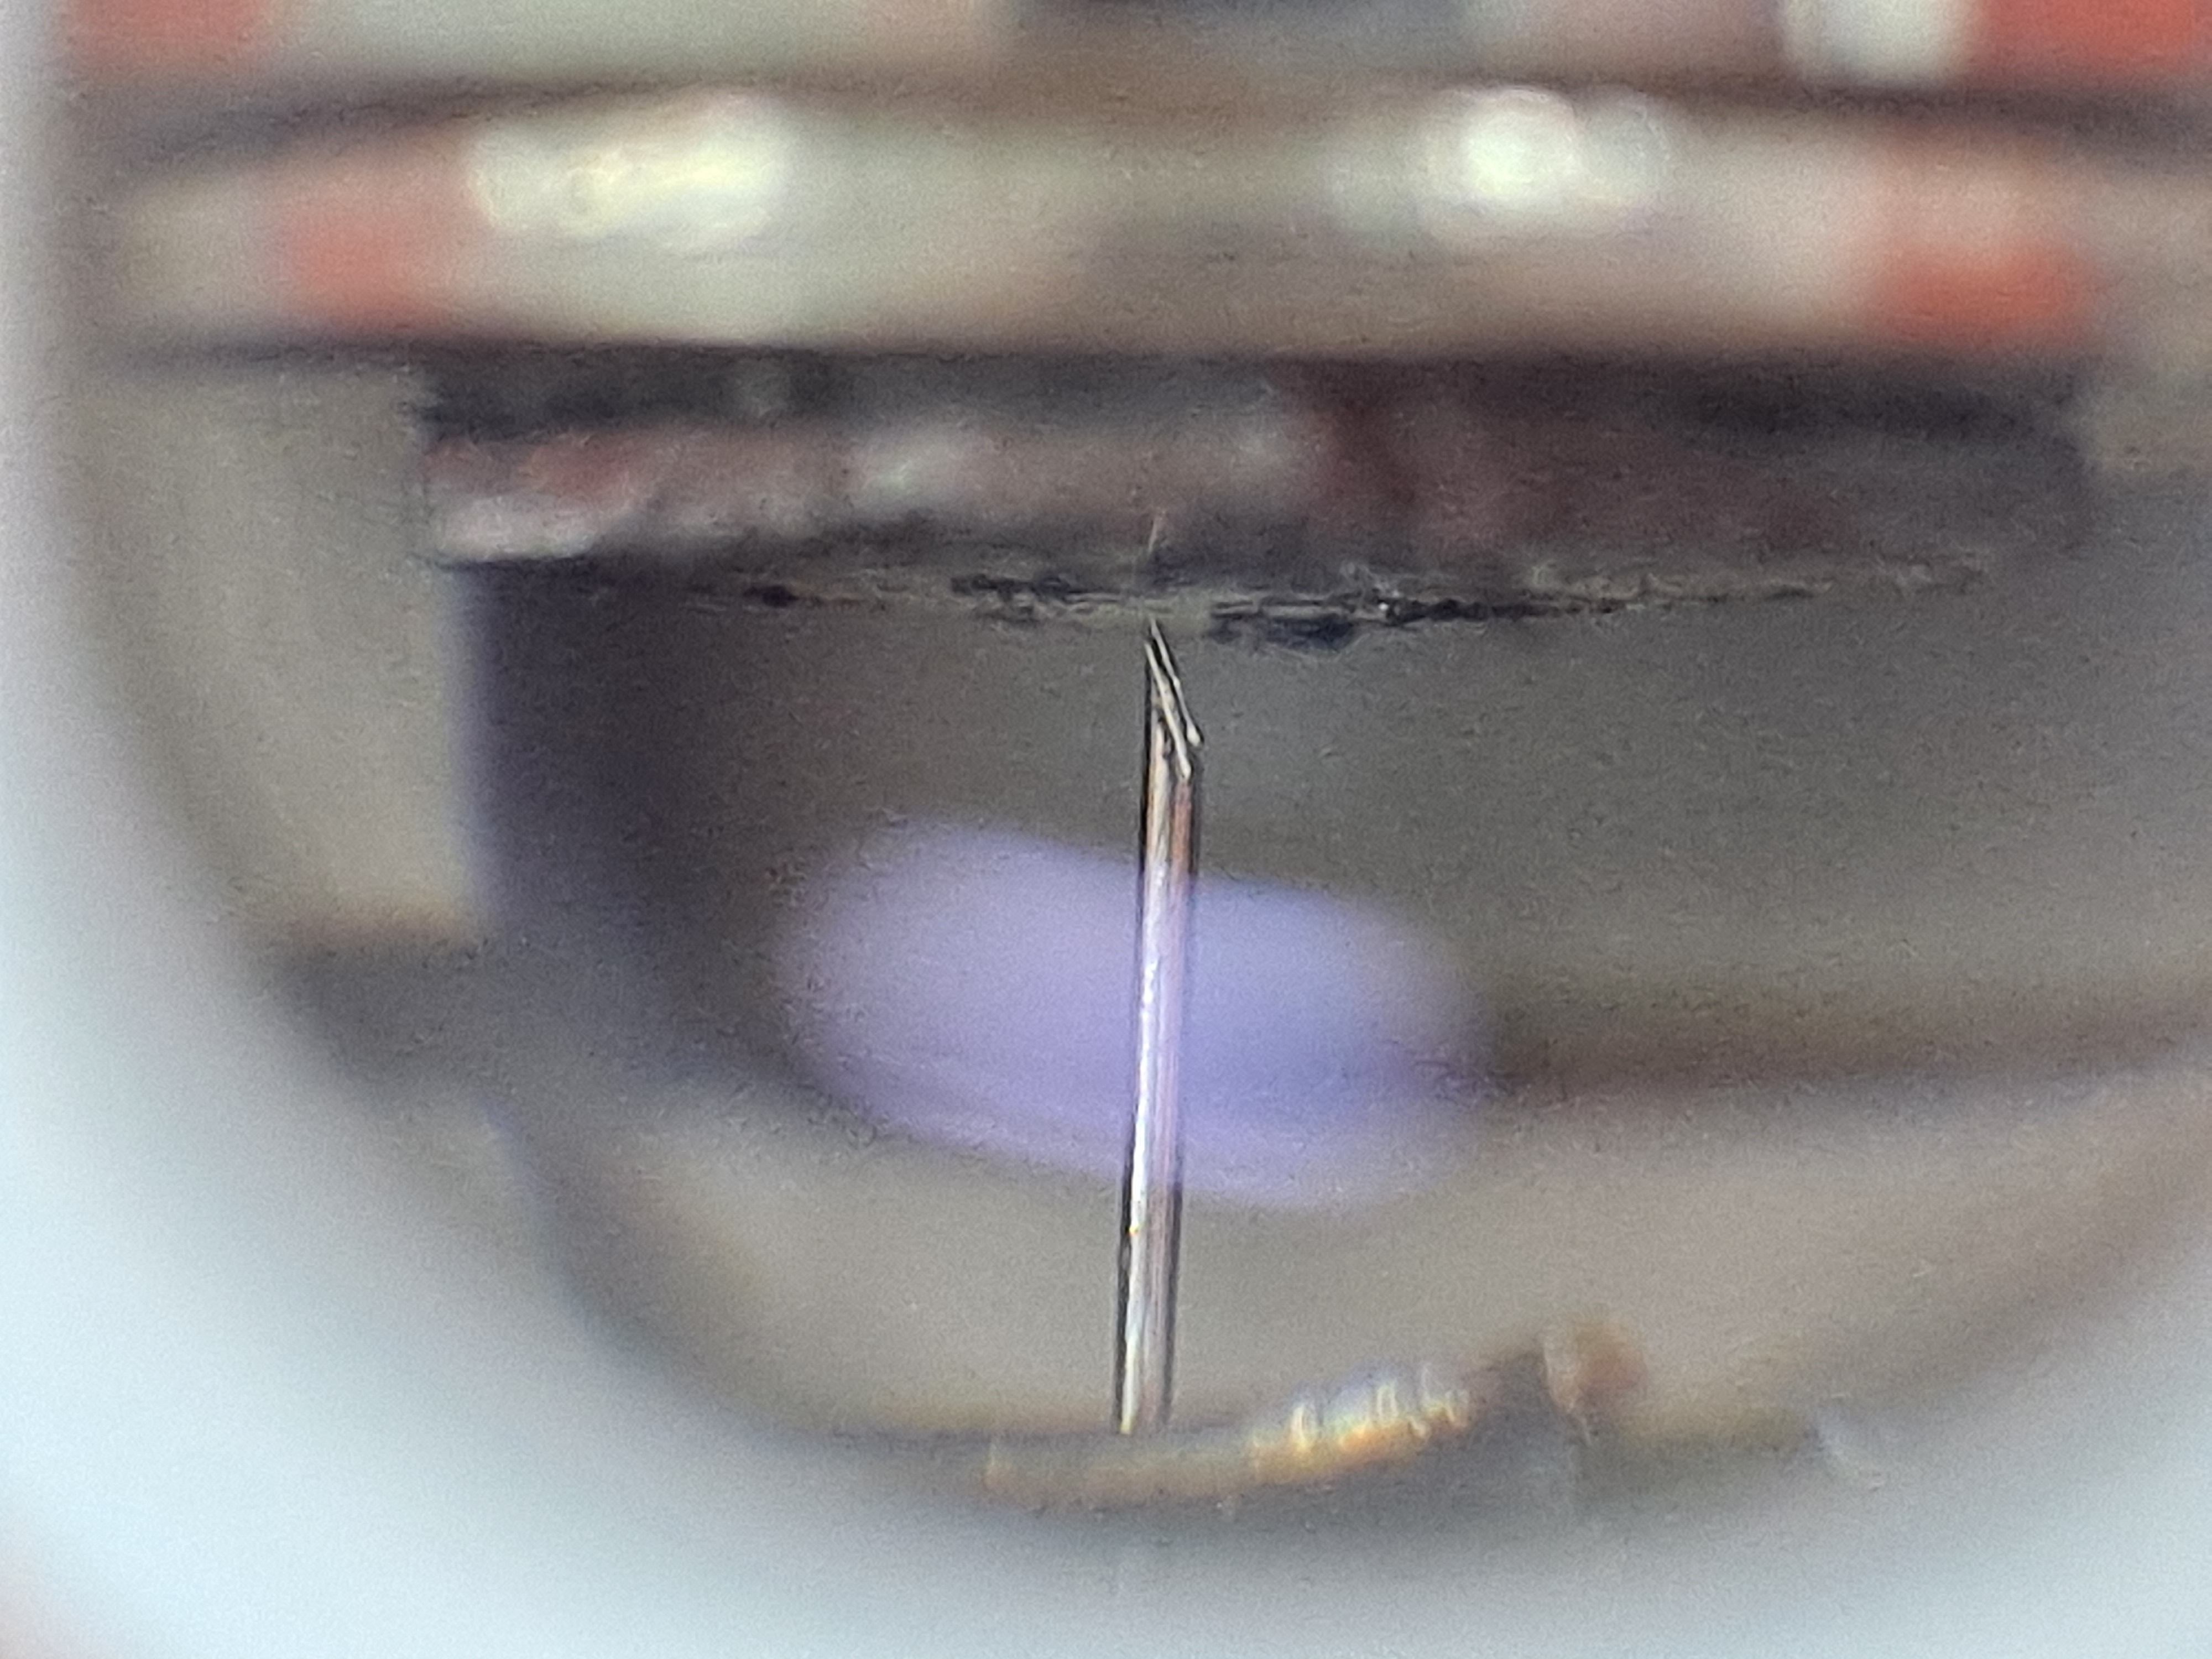
\includegraphics[width=5cm]{Figures/STM_TIP2.jpg}
				\captionof{figure}{Tip mounted on the STM.}
				\label{fig:STM_TIP2}
			\end{minipage}
		\end{figure}
		\item 뚜껑을 닫고 팁과 샘플과의 거리가 0.1 cm이내인지 확인한다.
		\item Magnifying cover를 덮고 the flat pliers와 기타 도구들을 정리한다.
	\end{enumerate}

%----------------------------------------------------------------------------------------
%	RESULT AND DISCUSSION
%----------------------------------------------------------------------------------------

\section{Result and Discussion}

	STM 측정 프로그램 셋팅을 다음과 같이 설정한다.
	
	\begin{table*}[htb!]
		\label{tab:2}
		\centering
		\resizebox{\textwidth}{!}{
		\begin{tabular*}{\textwidth}{@{\extracolsep{\fill}}ccc|ccc}
				\noalign{\smallskip}\noalign{\smallskip}\hline\hline
			& Size (nm) & & Point/Line & Time (s) \\
			\hline
			& 200 & & 128 & 0.2 \\
			& 2 & & 512 & 0.5 \\
			\hline
			\hline
		\end{tabular*}
		}
	\end{table*}

	Tip을 깎아서 장착 후, Sample HOPG를 장착한다. Sample의 적당한 위치에 맞춰 tip 위치를 조정한다. 프로그램을 사용하여 sample의 위치를 미세 조정한다.

	Advanced/Retract, approach/withdraw를 사용하여 Tunneling하는 순간까지 이동시킨다. Sample size에 맞춰 측정한다.

	\begin{figure}[htb!]
		\centering
		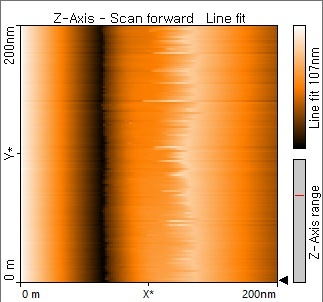
\includegraphics[width=5cm]{Figures/Scan_200nm.jpg}
		\caption{Scanned at 200 nm with HOPG.}
		\label{fig:Scan_200nm}
	\end{figure}

	200 nm로 측정했을 때, 미끄러지는 노이즈가 생겼다. 이렇게 될 경우, sample size를 줄이면 노이즈가 급격히 심해질 수 있다. (Figures~4)

	\begin{figure}[htb!]
		\centering
		\begin{minipage}{.5\textwidth}
			\centering
			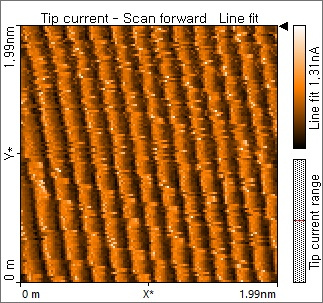
\includegraphics[width=5cm]{Figures/Scan_2nm_1.jpg}
			\label{fig:Scan_2nm1}
		\end{minipage}%
		\begin{minipage}{.5\textwidth}
			\centering
			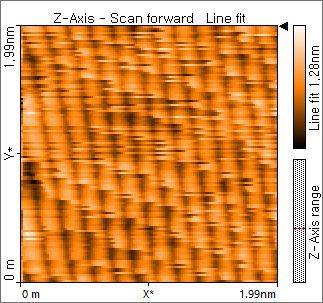
\includegraphics[width=5cm]{Figures/Scan_2nm_2.jpg}
			\label{fig:Scan_2nm2}
		\end{minipage}
		\caption{Scanned at 2 nm with HOPG.}
	\end{figure}

	2 nm로 측정했을 때, 분자 사이즈의 10배 정도의 size로 측정되기에 한 line에 10개 정도의 분자가 보일 것이다. HOPG는 Graphite이기에 육각형 튜브 구조이다. 측정이 잘 되었다면 육각형의 원자 구조를 볼 수 있었겠으나, tip이 잘 만들어지지 않아 노이즈가 생겨 Figures~5와 같이 육각 구조가 이어져 있는 line으로 보인다. (Figures~5)


	\begin{figure}[htb!]
		\centering
		\begin{minipage}{.5\textwidth}
			\centering
			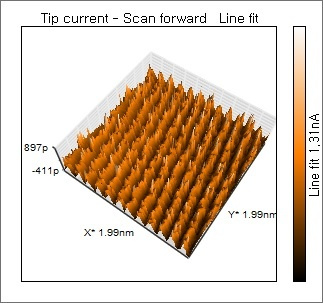
\includegraphics[width=5cm]{Figures/Scan_2nm_3D1.jpg}
			\label{fig:Scan_2nm_3D1}
		\end{minipage}
		\begin{minipage}{.5\textwidth}
			\centering
			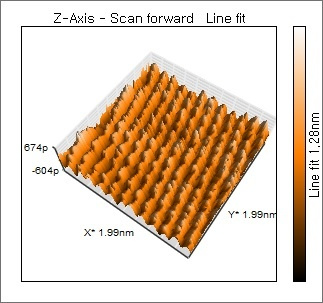
\includegraphics[width=5cm]{Figures/Scan_2nm_3D2.jpg}
			\label{fig:Scan_2nm_3D2}
		\end{minipage}
		\caption{3D scanned at 2nm with HOPG.}
	\end{figure}

	3D로 봤을 때는 2D linear 형태보다 잘 보임을 알 수 있다. Tunneling이 잘 되는 부분이 매우 잘 보인다. 다만 Figures~5와 같이 육각 구조가 보이지는 않았다. (Figures~6)

%----------------------------------------------------------------------------------------
%	CONCLUSIONS
%----------------------------------------------------------------------------------------

\section{Conclusions}

	STM을 사용하여 HOPG를 Scan하였을 때 대략적인 분자 구조를 확인할 수 있었으며, 3D model로 확인할 경우 tunneling을 볼 수 있었다. Tip을 더 잘 만들고, sample이 깨끗했다면 2 nm or below에서도 노이즈가 적게 측정되어 분자 구조가 보였을 것이다.

%----------------------------------------------------------------------------------------
%	FITTING CODE FOR PYTHON
%----------------------------------------------------------------------------------------

% \section{Fitting code for Python}

%----------------------------------------------------------------------------------------
%	BIBLIOGRAPHY
%----------------------------------------------------------------------------------------

% \printbibliography % Output the bibliography

%----------------------------------------------------------------------------------------

\end{document}